\section{  ANTICIPATED DATA PRODUCTS AND THEIR CHARACTERISTICS    }
\label{Sec:dataprod}

The LSST observing strategy is designed to maximize the scientific
throughput by minimizing slew and other downtime and by making appropriate
choices of the filter bands given the real-time weather conditions.
Using simulated surveys produced with the Operations Simulator described in \S~\ref{sec:opsim},
we illustrate predictions of LSST performance with two examples.


\subsection{ The Baseline LSST Surveys }
\label{sec:baseline}

The fundamental basis of the LSST concept is to scan the sky deep, wide, and
fast, and to obtain a dataset that simultaneously satisfies the majority
of the science goals. We present here a specific realization, the
so-called ``universal cadence'', which yields the main deep-wide-fast
survey and meets our core science goals.  However, at this writing,
there is a vigorous discussion of cadence plans in the LSST community,
exploring variants and alternatives that enhances various specific
science programs, while maintaining the science requirements described
in the SRD.

The main deep-wide-fast survey %(typical single visit depth of $r\sim24.5$)
will use about 90\% of the observing time. The remaining 10\% of the observing
time will be used to obtain improved coverage of parameter space such as
very deep ($r\sim26$) observations, observations with very short revisit
times ($\sim$1 minute), and observations of ``special'' regions such as the
Ecliptic, Galactic plane, and the Large and Small Magellanic Clouds.
We are also considering a third type of survey, micro-surveys, that would
use about 1\% of the time (which still represents 25 nights on a unique
8m-class telescope).

\subsubsection{ The Main Deep-Wide-Fast Survey }


\begin{figure}
%\includegraphics[width=1.0\hsize,clip]{rbandSky}
%\includegraphics[width=0.78\hsize,angle=90.0,clip]{rvisits_SciBook}
%\hskip -0.0in
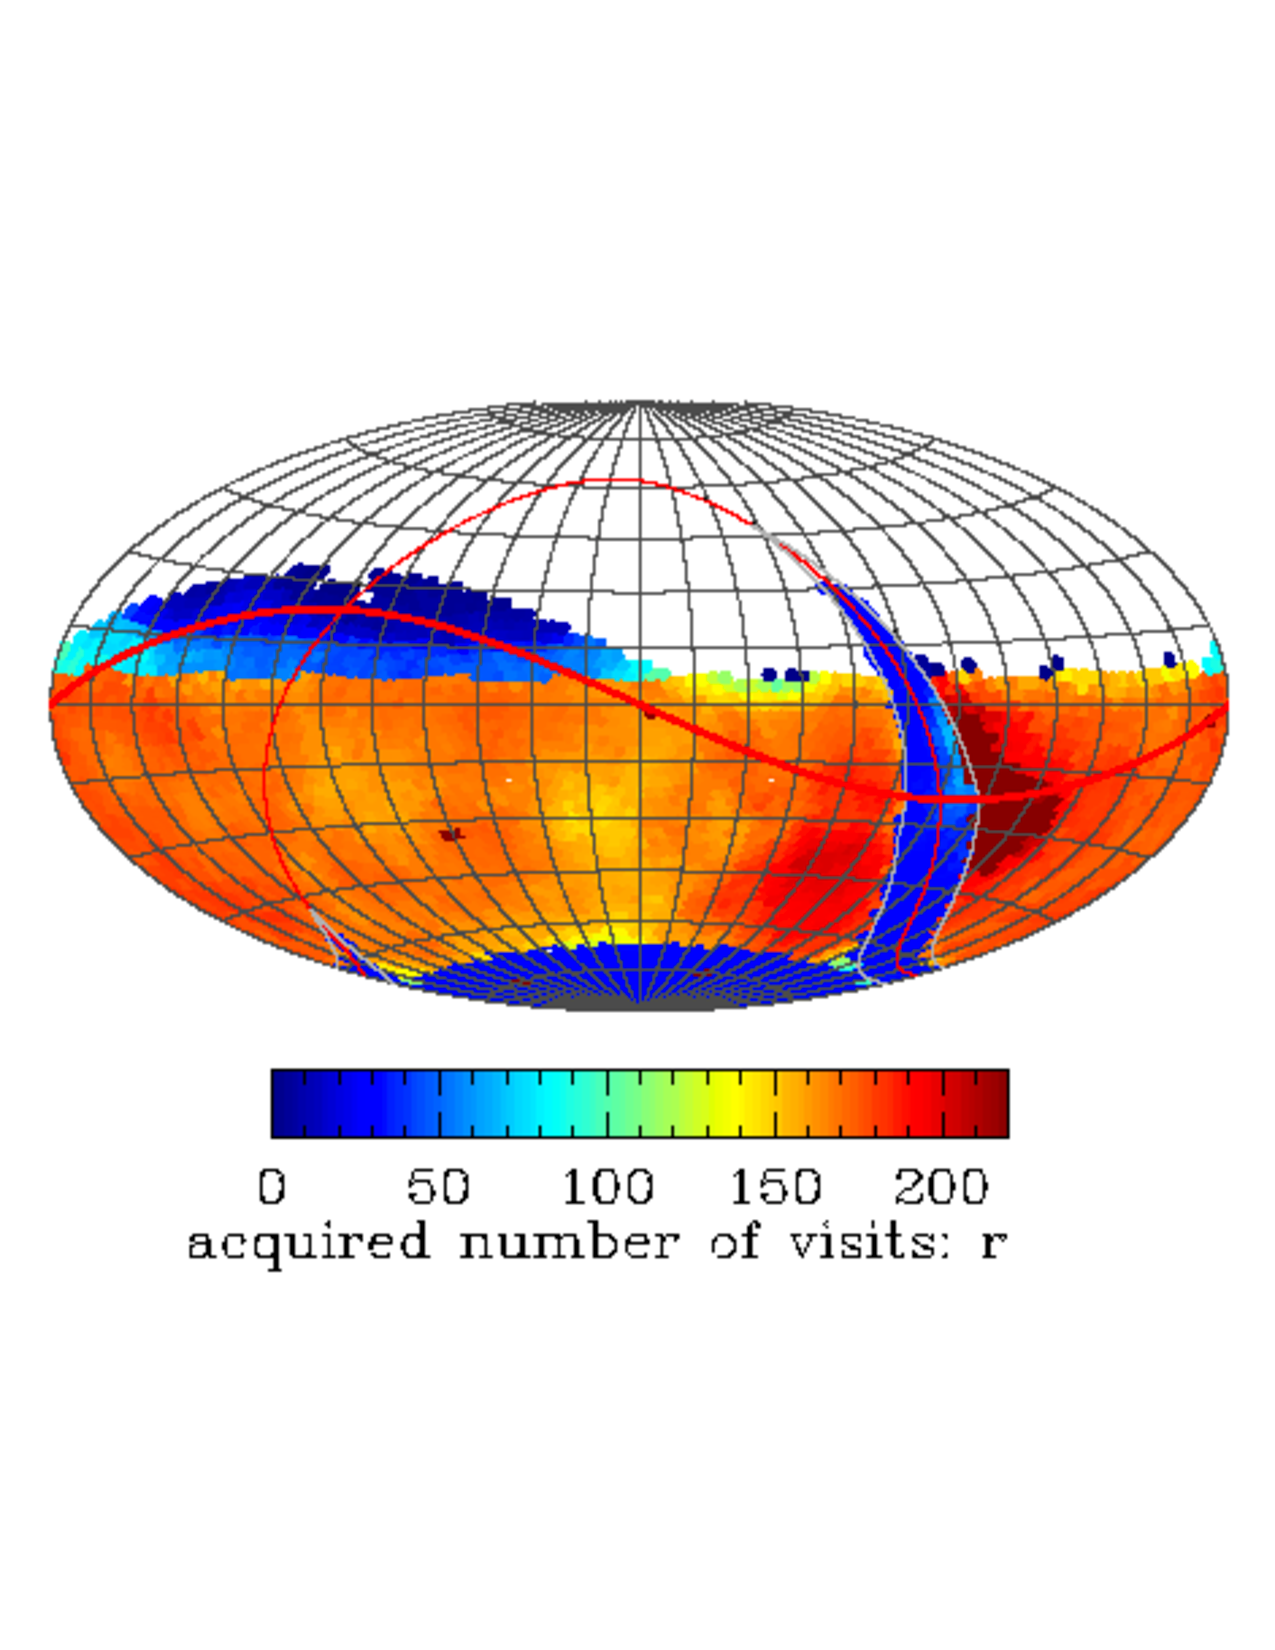
\includegraphics[width=1.0\hsize,clip]{rBandWhite}
\vskip -0.01in
\caption{The distribution of the $r$ band visits on the sky for a simulated
realization of the baseline cadence. The sky is shown in the equal-area Mollweide
projection in equatorial coordinates (the vernal equinoctial point is in the center, and
the right ascension is increasing from right to left). The number of visits for
a 10-year survey, normalized to the SRD design value of 184, is color-coded according
to the legend. The two regions with smaller number of visits than the main survey
(``mini-surveys'') are the Galactic plane (arc on the right) and the region around the
South Celestial Pole (bottom). The so-called ``northern Ecliptic region'' (upper left)
has received more visits than the main survey in this particular simulation (in
order to increase completeness for moving objects by increasing the coverage of
the Ecliptic plane). Deep drilling fields, with a much higher number of visits than
the main survey, are also visible as small circles. The fields were dithered on
sub-field scales and pixels with angular resolution of $\sim$30 arcmin were used
to evaluate and display the coverage.}
\label{Fig:rbandSky}
\end{figure}

The observing strategy for the main survey will be optimized for the homogeneity
of depth and number of visits. In times of good seeing and at low airmass, preference
is given to $r$-band and $i$-band observations. As often as possible, each field will be
observed twice, with visits separated by 15-60 minutes. This strategy will provide motion
vectors to link detections of moving objects in the Solar System, and fine-time sampling
for measuring short-period variability. The ranking criteria also ensure that the
visits to each field are widely distributed in position angle on the sky and
rotation angle of the camera in order to minimize systematic effects in galaxy shape
determination.

The universal cadence provides most of LSST's power for detecting Near Earth
Objects (NEO) and naturally incorporates the southern half of the ecliptic
within its 18,000 square degrees (the northern half lies above the desired airmass
limits, $X\la1.5$). NEO sample completeness for the smallest bodies ($\sim$140m in
diameter, per the Congressional NEO mandate) is greatly enhanced, however, by the
addition of a crescent on the sky within 10 degrees of the northern ecliptic
(see Fig.~\ref{Fig:rbandSky}). Thus, we plan to extend
%the ``northern Ecliptic proposal'' (here ``proposal'' refers to an observing program) extends
 the universal cadence to this region using the
$r$ and $i$ filters only, along
with more relaxed limits on airmass and seeing. Relaxed limits on airmass and
seeing are also adopted for $\sim$700 deg$^2$ around the South Celestial
Pole, allowing coverage of the Large and Small Magellanic Clouds.

Finally, the universal cadence proposal excludes observations in a region of
1,000 square degrees around the Galactic Center, where the high stellar
density leads to a confusion limit at much brighter magnitudes than those
attained in the rest of the survey. Within this region, the Galactic Center
proposal provides 30 observations in each of the six filters, distributed
roughly logarithmically in time (it may not be necessary to use the
$u$ and $g$ filters for this heavily extincted region).

The resulting sky coverage for the LSST baseline
cadence, based on detailed operations simulations, is shown for the
$r$ band in Fig.~\ref{Fig:rbandSky}. The anticipated total number of visits
for a ten-year LSST survey is about 2.8 million ($\sim$5.6 million 15-second long
exposures). The per-band allocation of these visits is shown in Table~\ref{tab:baseline}.



\subsubsection{ Mini-surveys}
\label{Sec:minisurveys}

Although the uniform treatment of the sky provided by the universal cadence
proposal can satisfy the majority of LSST scientific goals, roughly 10\%
of the time will be allocated to other strategies that significantly enhance the
scientific return.  These surveys aim to extend the parameter space accessible
to the main survey by going deeper or by employing different time/filter
sampling.

As an example of a mini-survey, consider a program that uses one hour of
observing time per night to observe a relatively small region of sky to
substantially greater depth in individual visits. Accounting for
read-out time and filter changes, it could obtain about 50 consecutive
15-second exposures in each of four filters in an hour. If a field is visited
every two days over four months, about 600 deg$^2$ can be observed with this
cadence over 10 years. Taking weather into account, the selected fields would
each have on average about 40 hour-long sequences of 200 exposures each. Each
observation in a sequence would have an equivalent 5-$\sigma$ depth of
$r\sim24.5$, and each filter subsequence when coadded would be 2 magnitudes
deeper than the main survey visits ($r\sim26.5$). When all 40 sequences and
the main survey visits are coadded, they would extend the depth to $r\sim28$.

This data set would be excellent for a wide variety of science programs. The
individual sequences would be sensitive to 1\% variability on hourly time
scales, allowing discovery of planetary eclipses. If these fields were selected
at Galactic latitudes of $|b|\sim30$ deg, they would include about 10 million
stars with $r<21$ observed with signal-to-noise ratio above 100 in each visit.
When subsequences from a given night were coadded, they would
provide dense time sampling to a faint limit of $r\sim26.5$ (assuming observations
in 4 bands, every 2 days over 120 days, and accounting for weather losses), and thus
enable deep searches
for SN, trans-Neptunian objects, and other faint transient, moving and
variable sources.  For example, the SN sample
would be extended to redshifts of $z\sim1.2$, with more densely sampled light
curves than obtained from the universal cadence. Such sequences would also
serve as excellent tests of our photometric calibration procedures.

The LSST has already selected four distant extragalactic survey fields\footnote{For
details, see \url{http://www.lsst.org/News/enews/deep-drilling-201202.html}}
that the project guarantees to observe as Deep Drilling Fields with deeper coverage
and more frequent temporal sampling than provided by the standard LSST observing
pattern. These fields (Elias S1, XMM-LSS, Extended Chandra Deep Field-South, and
COSMOS) are  well-studied survey fields with substantial existing multiwavelength
coverage and other positive attributes. These four fields are only the first chosen
for deep-drilling observations; more such fields will be chosen later.

The baseline universal cadence is by no means the definitive plan for the entire
survey. Rather, it represents a proof of concept that it is indeed possible to
design a universal cadence which addresses a wide variety of science goals in a nearly
optimal way. We are undertaking a vigorous and systematic research effort to explore
the enormously large parameter space of possible surveys. The
scientific commissioning period
will be used to test the usefulness of various observing modes and to explore
alternative strategies. Proposals from the community
%, through the science collaborations (see \S~\ref{Sec:community}),
for specialized cadences (such as mini-surveys and
micro-surveys) will also be considered.



\begin{deluxetable}{|r|r|r|r|r|r|r|}
\tablecaption{The Parameters From Eqs.~\ref{ggg} and \ref{m5} \textbf{XXX will be updated!}\label{tab:eqparams}}
\tablehead{
\colhead{} & \colhead{$u$}  &   \colhead{$g$}   & \colhead{$r$}   &  \colhead{$i$}  & \colhead{$z$}  & \colhead{$y$}
}
\startdata
   $m_\mathrm{sky}$\tablenotemark{a} &   22.9    & 22.3    & 21.2    & 20.5    & 19.6    &  18.6  \\
   $\theta$\tablenotemark{b}      &   0.77     &  0.73     & 0.70    & 0.67    &  0.65   &  0.63  \\
   $\gamma$\tablenotemark{c}      &   0.037   & 0.038    & 0.039   & 0.039   & 0.040   & 0.040 \\
    $k_m$\tablenotemark{d}        &    0.451  &  0.163   &  0.087  &  0.065   &  0.043   &  0.138 \\
    $C_m$\tablenotemark{e}        &   22.92   & 24.29    & 24.33   & 24.20   & 24.07   & 23.69 \\
    $m_5$\tablenotemark{f}        &   23.68     &   24.89    & 24.43     &  24.00   & 24.45    & 22.60  \\
 $\Delta C^{\infty}_m$\tablenotemark{g} &  0.67   &  0.21     &  0.11   &  0.08   &   0.05  &  0.04  \\
 $\Delta C_m(2)$\tablenotemark{h} &  0.24   &  0.09     &   0.05  &  0.04   &   0.03  &  0.02 \\
   $\Delta m_5$\tablenotemark{i}  &   0.21    & 0.15   & 0.14     &  0.13   & 0.13    & 0.15  \\
\enddata
\tablenotetext{^a}{The expected median zenith sky brightness at Cerro Pach\'on, derived from
           the median dark sky brightness observed by SDSS (AB mag arcsec$^{-2}$).}
\tablenotetext{^b}{The expected delivered median zenith seeing (arcsec). For larger
           airmass, $X$, seeing is proportional to $X^{0.6}$.}
\tablenotetext{^c}{The band-dependent parameter from Eq.~\ref{ggg}.}
\tablenotetext{^d}{Adopted atmospheric extinction.}
\tablenotetext{^e}{The band-dependent parameter from Eq.~\ref{m5}.}
\tablenotetext{^f}{The typical 5$\sigma$ depth for point sources at zenith, assuming exposure time of
          2$\times$15\,sec, and observing conditions as listed. For larger
          airmass the 5$\sigma$ depth is brighter; see the bottom row.}
\tablenotetext{^g}{The loss of depth due to instrumental noise (assuming 9\,e$^-$ per pixel and readout,
       and two readouts per visit).}
\tablenotetext{^h}{Additive correction to $C_m$ when exposure time is doubled from its fiducial value
          to 60\,sec.}
\tablenotetext{i}{The loss of depth at airmass of $X=1.2$ due to seeing degradation
                 and increased atmospheric extinction.}
\end{deluxetable}






\subsection{  Detailed Analysis of Simulated Surveys  }

As examples of analysis enabled by the Operations Simulator, we describe
determination of the completeness of the LSST NEO sample, and estimation
of errors expected for trigonometric parallax and proper motion measurements.
In both examples, the conclusions crucially depend on assumed signal-to-noise
ratios, described next.

\subsubsection{  Expected Photometric Signal-to-Noise Ratio }

The output of operations simulations is a data stream consisting of
a position on the sky and the time of observation, together with
observing conditions such as seeing and sky brightness. The expected
photometric error (the inverse of the signal-to-noise ratio) for a single visit
can be written as
\begin{equation}
         \sigma_1^2 = \sigma_{sys}^2 + \sigma_{rand}^2,
\end{equation}
where $\sigma_{rand}$ is the random photometric error and $\sigma_{sys}$ is
the systematic photometric error (includes errors due to, e.g., imperfect
modeling of the point spread function, but does not include errors in
absolute photometric zeropoint). The calibration system and procedures
are designed to maintain $\sigma_{sys}<0.005$ mag. Based on
SDSS experience \citep{2007AJ....134.2236S}, the random photometric error for
point sources, as
a function of magnitude, is well described\footnote{Eq.~\ref{ggg} can
be derived from $\sigma_{rand}=N/S$, where $N$ is noise and $S$ is signal,
and by assuming that $N^2 = N_o^2 + \alpha S$. The constants $N_o$ and
$\alpha$ can be expressed in terms of a single unknown constant $\gamma$
by using the condition that $\sigma_{rand}=0.2$ for $m=m_5$.} by
\begin{equation}
\label{ggg}
  \sigma_{rand}^2 = (0.04-\gamma)\, x + \gamma \, x^2 \,\,\, \mathrm{(mag^2),}
\end{equation}
with $x \equiv 10^{0.4\,(m-m_5)}$. Here $m_5$ is the 5$\sigma$ depth (for
point sources) in a given band, and $\gamma$ depends on the sky
brightness, readout noise, etc.
%Using the LSST exposure time
%calculator\footnote{Available at \url{http://dls.physics.ucdavis.edu/etc}.}
%\citep{Gee2007},
Detailed determination of the system throughput yields the values of $\gamma$
listed in Table~\ref{tab:eqparams}. The 5$\sigma$ depth for point sources is determined from
\begin{eqnarray}
\label{m5}
  m_5 = C_m + 0.50\,(m_{sky}-21) + 2.5\,\log_{10}(0.7/\theta) +  \nonumber \\
        + 1.25\,\log_{10}(t_{vis}/30) - k_m(X-1) \phantom{xxxxx}
\end{eqnarray}
where $m_{sky}$ is the sky brightness (AB mag arcsec$^{-2}$), $\theta$ is
the seeing (FWHM, in arcsec), $t_{vis}$ is the exposure time (seconds),
$k$ is the atmospheric extinction coefficient, and $X$ is airmass.


The constants $C_m$ depend on the overall throughput of the instrument
and are computed using currently the best available throughput estimates for
optical elements and sensors. The resulting $C_m$ values are listed in Table~\ref{tab:eqparams}
and in all six bands they imply single visit depths (also listed in Table~\ref{tab:eqparams}) in the range
between minimum and design specification values from the Science Requirements
Document listed in Table~\ref{tab:baseline}.
The differences in performance between LSST and, for example, SDSS are easily
understood\footnote{SDSS data
typically reach a 5$\sigma$ depth for point sources of $r=22.5$
with an effective aperture of $D=2.22$ m, an exposure time of $t_{vis}=54$
sec, the median $r$ band sky brightness of $r_{sky}=20.9$ mag arcsec$^{-2}$,
the median seeing of $\theta=1.5$ arcsec, and the median airmass of $X=1.3$.
%%% fix numbers: (aperture and throughout)
In comparison, the LSST loss of depth is 0.32 mag due to shorter exposures,
while the gains are 1.17 mag due to larger aperture, 0.83 mag due to better
seeing, 0.20 mag due to fainter sky, for the net gain of $\sim$1.9 mag.}.

The structure of eq.~\ref{m5} nicely illustrates decoupling between the system
sensitivity which is fully absorbed into $C_m$ and observing conditions
(system deployment parameters) specified by $m_{sky}$, $\theta$, $t_{vis}$, $k_m$
and $X$. The computation of $C_m$ listed in Table~\ref{tab:eqparams} assumed instrumental noise of
9 e$^-$ per pixel and per readout, which has by and large negligible effect on $m_5$ in
all bands except for the $u$ band. This loss of depth due to instrumental noise, $\Delta C^{\infty}_m$,
is listed in Table~\ref{tab:eqparams}; it also corresponds to additive correction to $C_m$ when the
exposure time $t_{vis} \rightarrow \infty$. To predict $5\sigma$ depths for
exposure time $\tau$ times longer that the fiducial $t_{vis} = 30$ sec., the
following correction has to be added to $C_m$ listed in Table~\ref{tab:eqparams}:
\begin{equation}
\label{eq:DCm}
 \Delta C_m(\tau) = \Delta C^\infty_m - 1.25\,\log_{10}\left[1 + {10^{(0.8 \, \Delta C^\infty_m)} - 1 \over \tau}  \right].
\end{equation}
Of course, $\Delta C_m(\tau=1)=0$. Again, this effect is only substantial in the $u$
band, as demonstrated by $\Delta C_m(\tau = 2)$ listed in Table~\ref{tab:eqparams}.

The loss of depth at the airmass of $X=1.2$ due to seeing degradation
and increased atmospheric extinction is listed in the last row in Table~\ref{tab:eqparams}. Note
that the uncertainty of limiting depth predictions due to unpredictable solar
activity (which influences the night sky brightness, \citet{2008A&A...481..575P}) is about
0.1-0.2 mag.




\subsubsection{   The NEO Completeness Analysis    }
\label{Sec:NEOc}
Detailed analyses of the LSST completeness for PHAs and NEOs are
described in \citet{2017arXiv171110621J}, \citet{2017AJ....154...12V,2017AJ....154...13V}, and \citet{2016AJ....151..172G}.
After accounting for differences in their input assumptions and models, each of these independent
works calculates a completeness value which is consistent within a few percent.
Here we briefly summarize the LSST project analysis carried out in \citet{2017arXiv171110621J}; this
approach is roughly the same for each of the studies mentioned above.

To assess the LSST completeness for PHAs, the PHA
population is represented by a sample of orbits taken from the Solar
System model of \citet{2007AAS...211.4721G}.
The simulated baseline survey is used to determine which PHAs are present in
each exposure and at what signal-to-noise ratio they were observed. In
addition to  seeing, atmospheric transparency, and sky background effects
(see eq.~\ref{m5}), the signal-to-noise computation takes into account losses
due to non-optimal detection filters and object trailing. Using mean asteroid reflectance
spectra \citep{2009Icar..202..160D}, combined with the LSST bandpasses (listed in Table~\ref{tab:eqparams}),
we calculate expected colors, assuming all PHAs are C type asteroids, of
$V-m = (-1.53, -0.28, 0.18, 0.29, 0.30, 0.30)$ for $m=(u, g, r, i, z, y)$ to transform
standard $V$ band magnitudes to the magnitudes expected in each filter.  Due to
very red $V-u$ colors, and the relatively bright limiting magnitude in the $y$
band, the smallest objects are preferentially detected in the $griz$ bands.
The correction for trailing is implemented by subtracting from the right-hand
side of eq.~\ref{m5}
\begin{eqnarray}
 \Delta m_5^\mathrm{trailing} & = &1.25\,\log_{10}\left(1+0.42 \, x^2 \right) \\
   x & = & {v \,t_{vis} \over 24 \, \theta},
\end{eqnarray}
where the object's velocity, $v$, is expressed in deg.~day$^{-1}$.
For the nominal exposure time of 30 seconds and $\theta=0.7$ arcsec, the loss of limiting
magnitude is 0.04 mag for $v=0.25$ deg.~day$^{-1}$, typical for objects in the main
asteroid belt, and 0.46 mag for $v=1.0$ deg.~day$^{-1}$, typical of NEOs passing
near Earth. The PHA orbits are cloned over an $H$ magnitude distribution with $dN/dH = 10^{\alpha \, H}$,
with $\alpha=0.33$, in order to evaluate completeness as a function of $H$.

An object is considered to be discovered if the object was detected on at least three nights within a
window of 15 days, with a minimum of two visits per night. The same criterion has been used in NASA studies,
and is confirmed as reliable by a detailed analysis of orbital linking and orbit determination using the Moving
Object Processing System (MOPS) code \citep{2017AJ....154...12V,2017AJ....154...13V,2005AAS...20712102J} developed by the
Pan-STARRS project (and adopted by LSST in a collaborative effort with Pan-STARRS). The MOPS software
system and its algorithms are significantly more advanced than anything previously
fielded for this purpose to date. Realistic MOPS simulations show
$>$99\% linking efficiency across all classes of Solar System objects \citep{2013PASP..125..357D},
and at least 93\% efficiency for NEOs \citep{2017AJ....154...12V,2017AJ....154...13V}.

The LSST baseline cadence discovers 66\% of PHAs with $H\leq22$ (equivalent to $D\ge140$~m)
after 10 years of operations (61\% of NEOs with $H\leq22$) \citep{2017arXiv171110621J}.  This cadence spends 6\% of the total
observing time on NEO-optimized observations north of $\delta = +5^\circ$, and MOPS links objects with windows of 15 days.
The baseline survey cumulative completeness as a function of time for objects with $H\le22$ is shown in the upper panel of Fig.~\ref{Fig:Cneo},
both with and without including other surveys. These figures are likely to be uncertain to the level of $\pm5\%$ due
to unknown variations in the orbital distribution of the true population, the size distribution, uncertain distributions of shape
(and thus light curve variations) and surface properties (thus colors and albedo), plus variations in survey cadence due to
weather, etc.

\begin{figure}
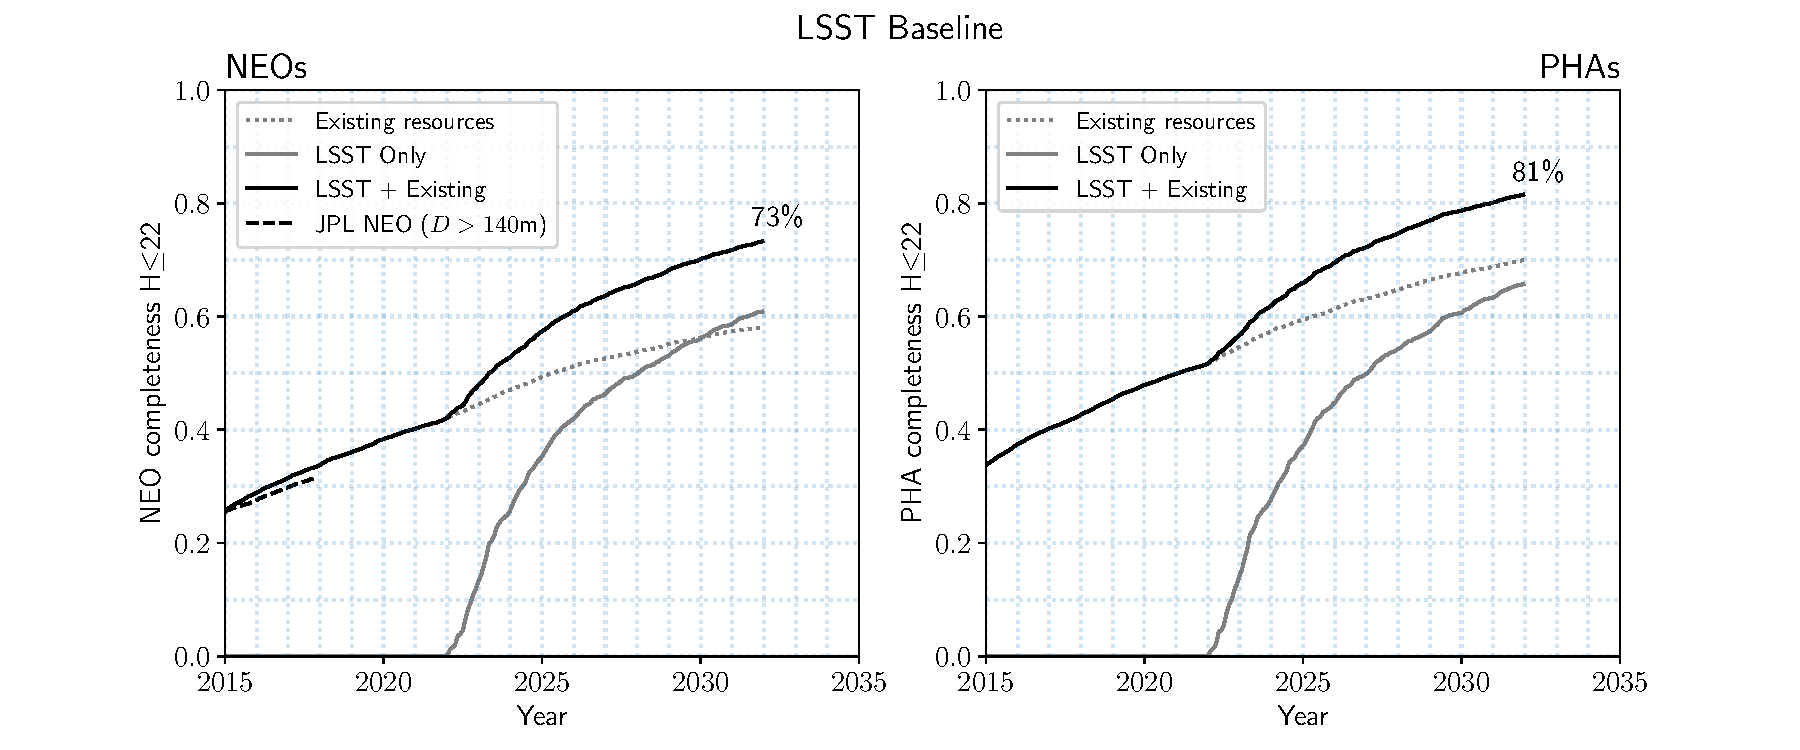
\includegraphics[width=1.\hsize,clip]{neo_pha_completeness_3in15_minion_1016}
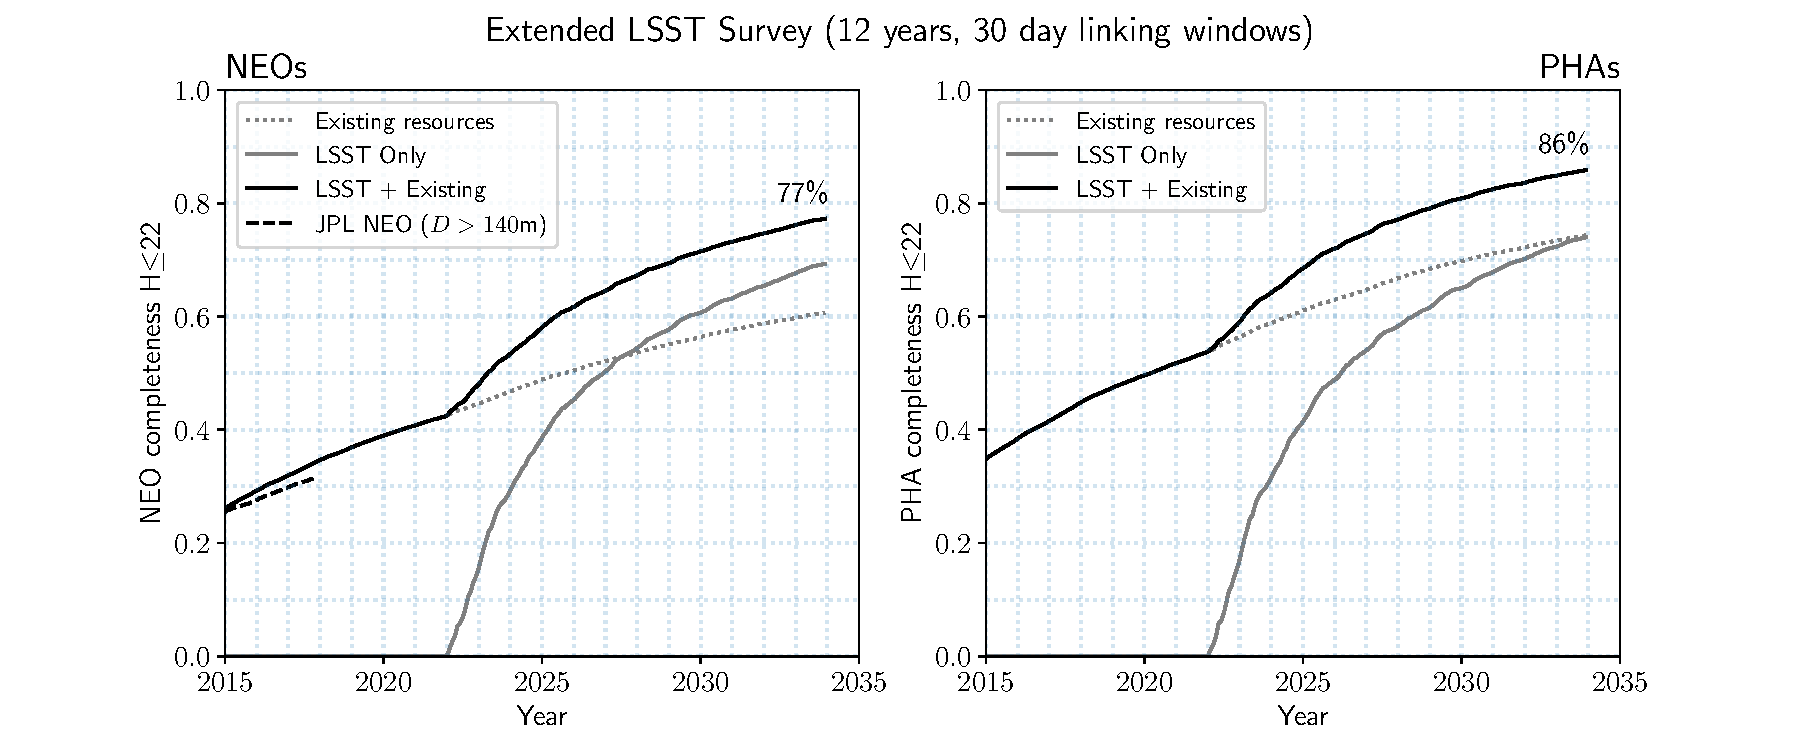
\includegraphics[width=1.\hsize,clip]{neo_pha_completeness_3in30_astro_lsst_01_1016}
\caption{Cumulative completeness of the LSST survey for NEOs (left in each panel) and PHAs (right in each panel)
brighter than a given absolute magnitude, $H\le22$ (related to the size of the object and albedo;
$H$=22 mag is equivalent to a typical 140m asteroid). The top panel illustrates cumulative completeness
for the LSST baseline cadence and MOPS configuration. In the baseline, LSST alone would discover 66\% of the PHAs
with $H\le22$ (61\% of NEOs); LSST combined with existing resources (including reasonable boosts
in capability in the future) can discover 81\% of PHAs (73\% of NEOs). The bottom panel illustrates cumulative
completeness when LSST is operated for 12 years, with extra visits around the ecliptic, and when the MOPS linking
window is increased to 30 days from the baseline 15. In this case, LSST alone could discover 74\% of the PHAs with
$H\le22$ (69\% of NEOs); LSST combined with existing resources could discover 86\% of PHAs (77\% of NEOs).
}
\label{Fig:Cneo}
\end{figure}

Various adjustments to the baseline cadence and MOPS can boost the completeness for $H\le22$ PHAs.
By improving MOPS and increasing the MOPS linking window from 15 to 30 days we can boost completeness
by about 3\%. By running the survey for an additional two years, we can boost completeness by another 4\%.
Considering this `extended' LSST in the context of existing/ongoing surveys would result in a system-wide cumulative completeness of 86\% for PHAs (77\% for NEOs), approaching the 90\% required by the Congressional mandate (see
lower panels of Fig.~\ref{Fig:Cneo}).

\subsubsection{The Expected Accuracy of Trigonometric Parallax and Proper Motion Measurements }
\label{sec:astrom}

Given the observing sequence for each sky position in the main survey, we
generate a time sequence of mock astrometric measurements. The assumed astrometric
accuracy is a function of signal-to-noise ratio. Random astrometric errors per
visit are modeled as $\theta/SNR$, with $\theta=700$ mas and $SNR$ determined using
eq.~\ref{m5}. The estimated proper motion and parallax accuracy at the bright end
($r<20$) is driven by systematic errors due to the atmosphere. Systematic
errors of 10 mas are added in quadrature, and are assumed to be {uncorrelated}
between different observations of a given object. Systematic and random
errors become similar at about $r=22$, and there are about 100 stars per LSST
sensor (0.05 deg$^2$) to this depth (and fainter than the LSST saturation limit at
$r\sim16$) even at the Galactic poles.

Data from the Subaru telescope reduced with the LSST software stack indicate that systematic errors of
10 mas on spatial scales of several arcminutes are realistic even at this stage of maturity of the
code; results reported by DES \citep{2017PASP..129g4503B} indicate astrometric residuals of $\sim 7$mas for 30s exposures
in a 4m, with scope for further improvements from denser astrometric standard grids. Even a drift-scanning
survey such as SDSS delivers uncorrelated systematic errors (dominated by seeing
effects) at the level of 20-30 mas \citep[measured from repeated scans;][]{2003AJ....125.1559P};
the expected image quality for LSST will be twice as good as for SDSS. Furthermore,
there are close to 1000 galaxies per sensor with $r<22$, which will provide exquisite
control of systematic astrometric errors as a function of magnitude, color and other
parameters, and thus enable absolute proper motion measurements.



\begin{deluxetable}{l|c|c|c|c|c}
\tablecaption{The expected proper motion, parallax and accuracy for a 10-year long baseline survey.\label{tab:tenyear}}
\tablehead{
\colhead{$r$} &  \colhead{$\sigma_{xy}$\tablenotemark{a}} & \colhead{$\sigma_\pi$\tablenotemark{b}} & \colhead{$\sigma_\mu$\tablenotemark{c}} & \colhead{$\sigma_1$\tablenotemark{d}} &  \colhead{$\sigma_C$\tablenotemark{e}} \\
\colhead{mag} & \colhead{mas} & \colhead{mas} & \colhead{mas/yr} & \colhead{mag} & \colhead{mag}
}
\startdata
       21 &  11  &  0.6  &  0.2   &   0.01  &   0.005 \\
       22 &  15  &  0.8  &  0.3   &   0.02  &   0.005 \\
       23 &  31  &  1.3  &  0.5   &   0.04  &   0.006 \\
       24 &  74  &  2.9  &  1.0   &   0.10  &   0.009 \\
\enddata
\tablenotetext{a}{Typical astrometric accuracy (rms per coordinate per visit).}
\tablenotetext{b}{Parallax accuracy for 10-year long survey.}
\tablenotetext{c}{Proper motion accuracy for 10-year long survey.}
\tablenotetext{d}{Photometric error for a single visit (two 15-second exposures).}
\tablenotetext{e}{Photometric error for coadded observations (see Table~\ref{tab:baseline}).}
\end{deluxetable}


The astrometric transformations for a given CCD and exposure, and
proper motion and parallax for all the stars from a given CCD, are simultaneously
solved for using an iterative algorithm. The astrometric transformations from
pixel to sky coordinates are modeled using low-order polynomials and standard
techniques developed at the U.S. Naval Observatory \citep{2003AJ....125..984M}. The expected
proper motion and
parallax errors for a 10-year long baseline survey, as a function of apparent
magnitude, are summarized in Table~\ref{tab:tenyear}. Blue stars (e.g., F/G stars) fainter than
$r\sim23$ will have about 50\% larger proper motion and parallax errors than
given in the table due to decreased numbers of $z$ and $y$ band detections. The
impact on red stars is smaller due to a relatively small number of observations
in the $u$ and $g$ bands, but extremely red objects, such as L and T dwarfs,
will definitely have larger errors, depending on details of their spectral
energy distributions.  After the first three years of the survey,
{the proper motion errors will be about five times as large, and parallax
errors will be about twice as large,} as the values given in Table~\ref{tab:tenyear}; the errors
scale as $t^{-3/2}$ and $t^{-1/2}$, respectively. This error behavior is
a strong independent argument for a survey lifetime of at least 10 years
(c.f. \S 2).





For comparison with Table~\ref{tab:tenyear}, the SDSS-POSS proper motion measurements have an
accuracy of $\sim$5 mas yr$^{-1}$ per coordinate at $r=20$ \citep{2004AJ....127.3034M}. Gaia
is expected to deliver parallax errors of 0.3 mas and proper motion errors of
0.2 mas yr$^{-1}$ at its faint end at $r\sim20$ \citep{2001A&A...369..339P}. Hence, LSST will smoothly
extend Gaia's error vs.\ magnitude curve 4 magnitudes fainter.


\subsection{             Data Products and Archive Services          }
\label{Sec:dp}

Data collected by the LSST telescope and camera will be automatically processed to \emph{data products} -- catalogs, alerts,
and reduced images -- by the LSST Data Management system
(\S~\ref{sec:dm}). These products are designed to be sufficient to
enable a large majority of LSST science cases, without the need to
work directly with the raw pixels.  We give a high-level overview of
the LSST data products here; further details may be found in the LSST
Data Products Definition Document \citep{LSE-163}.

\vskip 1em

Two major categories of data products will be produced and delivered by LSST DM:
\begin{itemize}
\item \textbf{  Prompt products\footnote{Historically, these have been referred to as ``Level
1 Data Products'', but going forward we prefer to use the more descriptive
\emph{Prompt Products} designation. Note that the old terminology is still
in use in present-day LSST documents and code; new and updated
documents will gradually transition to the new, descriptive, nomenclature
used in this paper.
}}, designed to support the discovery,
  characterization, and rapid follow-up of time-dependent phenomena
  (``transient science''). These will be generated continuously every
  observing night, by detecting and characterizing sources in images
  differenced against deep templates. They will include alerts to
  objects that were newly discovered, or have changed brightness or
  position at a statistically significant level. The alerts to such
  events will be published within 60   seconds of observation.\\
\\
In addition to transient science, the prompt products will support
discovery and follow-up of objects in the Solar System. Objects with
motions sufficient to cause trailing in a single exposure will be
identified and flagged as such when the alerts are broadcast. Those
that are not trailed will be identified and linked based on their
motion from observation to observation, over a period of a few
days. Their orbits will be published within 24 hours of
identification. The efficiency of linking (and thus the completeness
of the resulting orbit catalog) will depend on the final observing
cadence chosen for LSST, as well as the performance of the linking
algorithm (\S~\ref{Sec:NEOc}).
\item \textbf{Data release products\footnote{These have been referred to as ``Level
2 Data Products'' in the past; as with their ``Level 1`` counterparts, we
will use the more descriptive nomenclature going forward.}} are designed to enable systematics- and flux-limited science, and will be made available in generally annual Data Releases. These will include the (reduced and raw) single-epoch images, deep coadds of the observed sky, catalogs of objects detected in LSST data, catalogs of sources (the detections and measurements of objects on individual visits), and catalogs of ``forced sources" (measurements of flux on individual visits at locations where objects were detected by LSST or other surveys). LSST data releases will also include fully reprocessed prompt products, as well as all metadata and software necessary for the end-user to reproduce any aspect of LSST data release processing.\\
\\
A noteworthy aspect of LSST data release processing is that it will largely
rely on \textbf{multi-epoch model fitting}, or \textbf{\emph{MultiFit}}, to
perform near-optimal characterization of object properties. That is,
while the coadds will be used to perform object \emph{detection}, the
\emph{measurement} of their properties will be performed by
simultaneously fitting (PSF-convolved) models to single-epoch
observations. It is not yet clear to what extent we will be able to make some of these
measurements on suitable linear combinations of input images (with careful propagation
of PSFs and noise).
An extended source model -- a constrained linear
combination of two S\'ersic profiles -- and a point source model with
proper motion -- will generally be
fitted to each detected object\footnote{For performance reasons, it is
  likely that only the point source model will be fitted in the most
  crowded regions of the Galactic plane.}.\\
\\
Secondly, for the extended source model fits, the LSST will
characterize and store the shape of the associated likelihood surface
(and the posterior), and not just the maximum likelihood values and
covariances. The characterization will be accomplished by sampling,
with up to $\sim$200 (independent) likelihood samples retained for
each object. For storage cost reasons, these samples
may be retained only for those bands of greatest interest for
weak lensing studies.

\end{itemize}

We have described that approximately 10\% of the observing time will
be devoted to mini-surveys that do not follow the LSST baseline
cadence (\S~\ref{Sec:minisurveys}). The data products for these
programs will be generated using the same processing system and
exhibit the same general characteristics of prompt or data release   data
products, but these data may be reduced on a somewhat different
timescale.

While a large majority of science cases will be adequately served by prompt
and data release products, more specialized investigations may benefit from
custom, user-created, products derived from the LSST data.  These could be
new catalogs created by simple post-processing of the LSST data release
catalogs, entirely new data products generated by running custom code on raw
LSST imaging data, or something in-between.  We will make it possible for the
end-users to create (or use) such \textbf{user generated\footnote{Formerly known as
``Level 3 Data Products``.}} products at the LSST Large Data Facility,
using the services offered within the LSST Science Platform (\S~\ref{sec:lsp}).


\subsubsection{The LSST Science Platform}
\label{sec:lsp}

The LSST Science Platform \citep{LSE-319} represents LSST's vision for a
large-scale astronomical data archive that can enable effective research
with datasets of LSST size and complexity.  It builds on recent trends in
remote data analysis, and practical experiences in the astronomical context
gathered by projects such as the JHU
SciServer \citep{2017AAS...22923615R}, Gaia GAVIP \citep{2016SPIE.9913E..1VV}, or NOAO Datalab \citep{2016SPIE.9913E..0LF}.

The LSST Science Platform will be a set of web applications (portals) and
services through which the users will access the LSST data products and, if
desired, conduct remote analyses or create user generated products.  The
platform makes this possible through tree user-facing \emph{aspects}:
%
\begin{itemize}

\item The web \textbf{Portal}, designed to provide the essential data access and
visualization services through a simple-to-use website.  It will enable
querying and browsing of the available datasets in ways the users are
accustomed to at archives such as IRSA, MAST, or the SDSS archive.

\item The \textbf{JupyterLab} aspect, that will provide a
Jupyter\footnote{\url{http://jupyter.org/}} Notebook-like
interface and is geared towards enabling next-to-the-data remote analysis.
A large suite of commonly used astronomical software, including the LSST
software stack (\S~\ref{sec:dmstack}), will be made available through this
interface.  The user experience will be nearly identical to working with
Jupyter notebooks locally, except that computation and analysis will occur
with resources provided at the LSST Data Access Center.  This is an
implementation of the ``bringing computation to the data'' paradigm: rather
than imposing the burden of downloading, storing, and processing
(potentially large) subsets of LSST data at their home institutions, we make
it possible for the users to bring their codes and perform analyses at the
LSST DAC.  This reduces the barrier to entry and shortens the path to
science for the LSST science community.

\item The \textbf{Web API} aspect will expose the LSST DAC services to other
software tools and services using commonly accepted formats and protocols\footnote{For
example, industry-standard protocols such as WebDAV may be used to expose
file data, or Virtual Observatory protocols for access to catalogs or images
(TAP and SIAP, respectively), etc.}.  This interface will open the
possibility for remote access and analysis of the LSST data set using
applications that the users are already comfortable with such as
TOPCAT \citep{2005ASPC..347...29T}, or libraries such as Astropy \citep{2013A&A...558A..33A}.  Furthermore, the offered APIs will allow
for federation with other astronomical archives, bringing added value to the
LSST dataset.
\end{itemize}

Approximately 10\% of the total budget for the LSST Large Data Facility
compute and storage capacity has been reserved for the LSST Science Platform
needs, and to be shared by all LSST DAC users.  Based on the current plans and
technology projections, these equate to approximately 2,400 cores, 4 PB of
file storage, and 3 PB of database storage at the beginning of LSST
operations (in 2022).


\B{
\subsection{Data Mining Challenges}

The characterization (unsupervised machine learning) and classification (supervised machine learning) of
massive, multivariate data catalogs such as those generated by the LSST are major research challenges for
data-intensive astronomy
\citep{Tyson2008,2008AIPC.1082..359I,2008AN....329..284B,2008AN....329..255B,2014sdmm.book.....I}.
To address these questions, the statistics and machine-learning research
communities are collaborating with LSST scientists to develop new algorithms that will enable the full
scientific potential of the LSST, including:
\begin{itemize}
\item Rapid characterizations and probabilistic classifications for
  the million sources
          detected in difference images each night.
\item Identification of unusual classes of astronomical sources using outlier detection techniques that are
          robust to noise and image processing defects.
\item Characterization of novel and unexpected behavior in the time domain from time series data.
\item Measurements of the clustering of stars and galaxies (including higher order statistics) using fast
          algorithms for point processes.
\item The application of dimensionality-reduction techniques to determine important physical correlations
          within large multi-variate catalogs.
\item Model or hypothesis testing that can verify existing (or generate new) astronomical hypotheses with
          strong statistical confidence, using millions of training samples.
\end{itemize}

%The broad range of science that will benefit from statistically
%rigorous and computationally efficient algorithms has led to the
%creation of the Informatics and Statistical Science Research
%Collaboration for the LSST (see \S~\ref{Sec:community}) . This
%collaboration's goal is to develop, implement, and validate data
%mining algorithms that will scale to the size and complexity of the
%LSST data.
}




\begin{figure}
\begin{center}
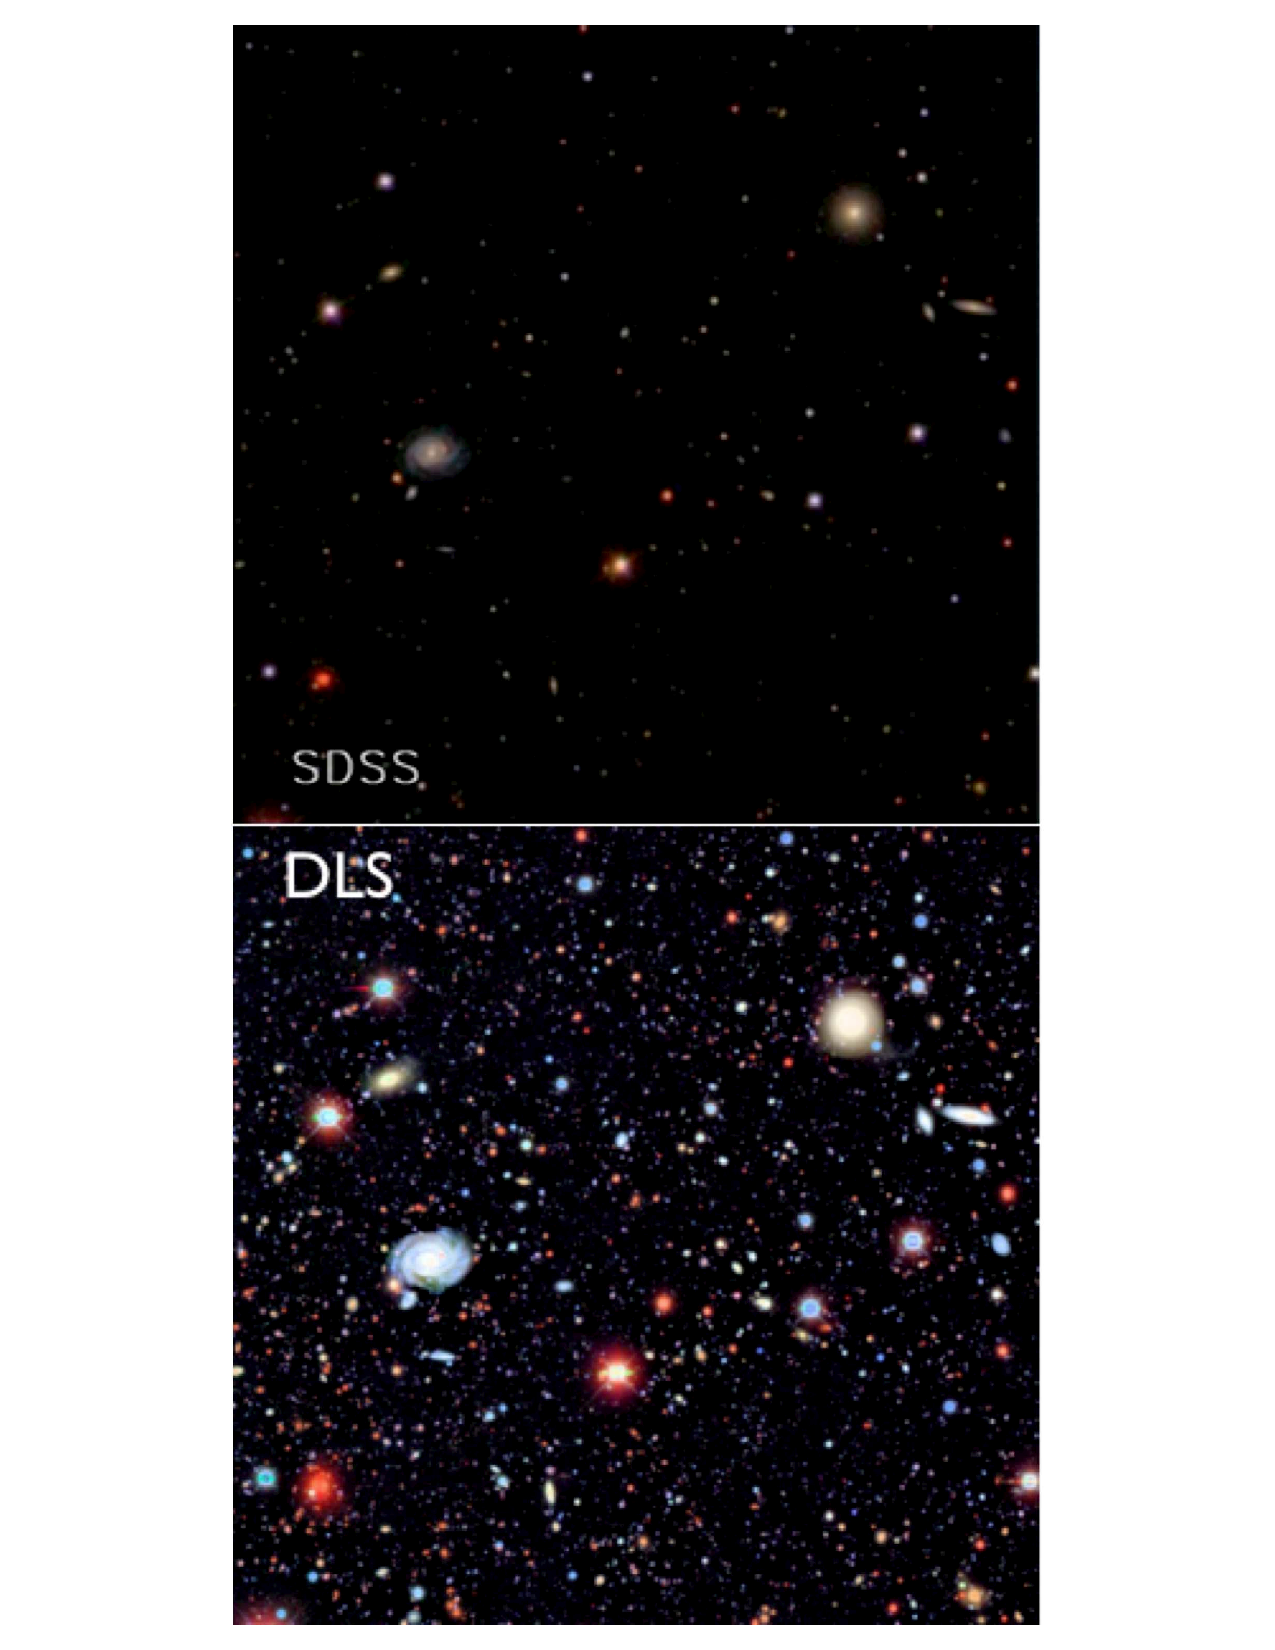
\includegraphics[width=0.47\textwidth,clip]{panels1_2}
\end{center}
\caption{A comparison of $\sim7.5\times7.5$ arcmin$^2$ images of
the same area of sky (centered on $\alpha$=9$^h$ 20$\arcmin$ 47$\arcsec$ and
$\delta$=30$^\circ$ 8$\arcmin$ 12$\arcsec$) obtained by the SDSS (top, $r<22.5$) and
the Deep Lens Survey (bottom, $r<24.5$). These are gri composites,
colorized following \citet{2004PASP..116..133L}.  The depth gain for the bottom image
is mostly due to the lower surface brightness limit, which is also responsible
for the apparent increase of galaxy sizes. LSST will obtain $\sim$100 $gri$
color images to the same depth ($\sim$200 for the $riz$ composites) of each point
over half the Celestial sphere (18,000 deg$^2$, equivalent to 1.15 million $\sim7.5\times7.5$
arcmin$^2$ regions), and with better seeing. After their coaddition, the final
image will be another $\sim3$ mag deeper (a faint limit of $r=27.5$ for point
sources).}
\label{Fig:panels1}
\end{figure}

\begin{figure}
\begin{center}
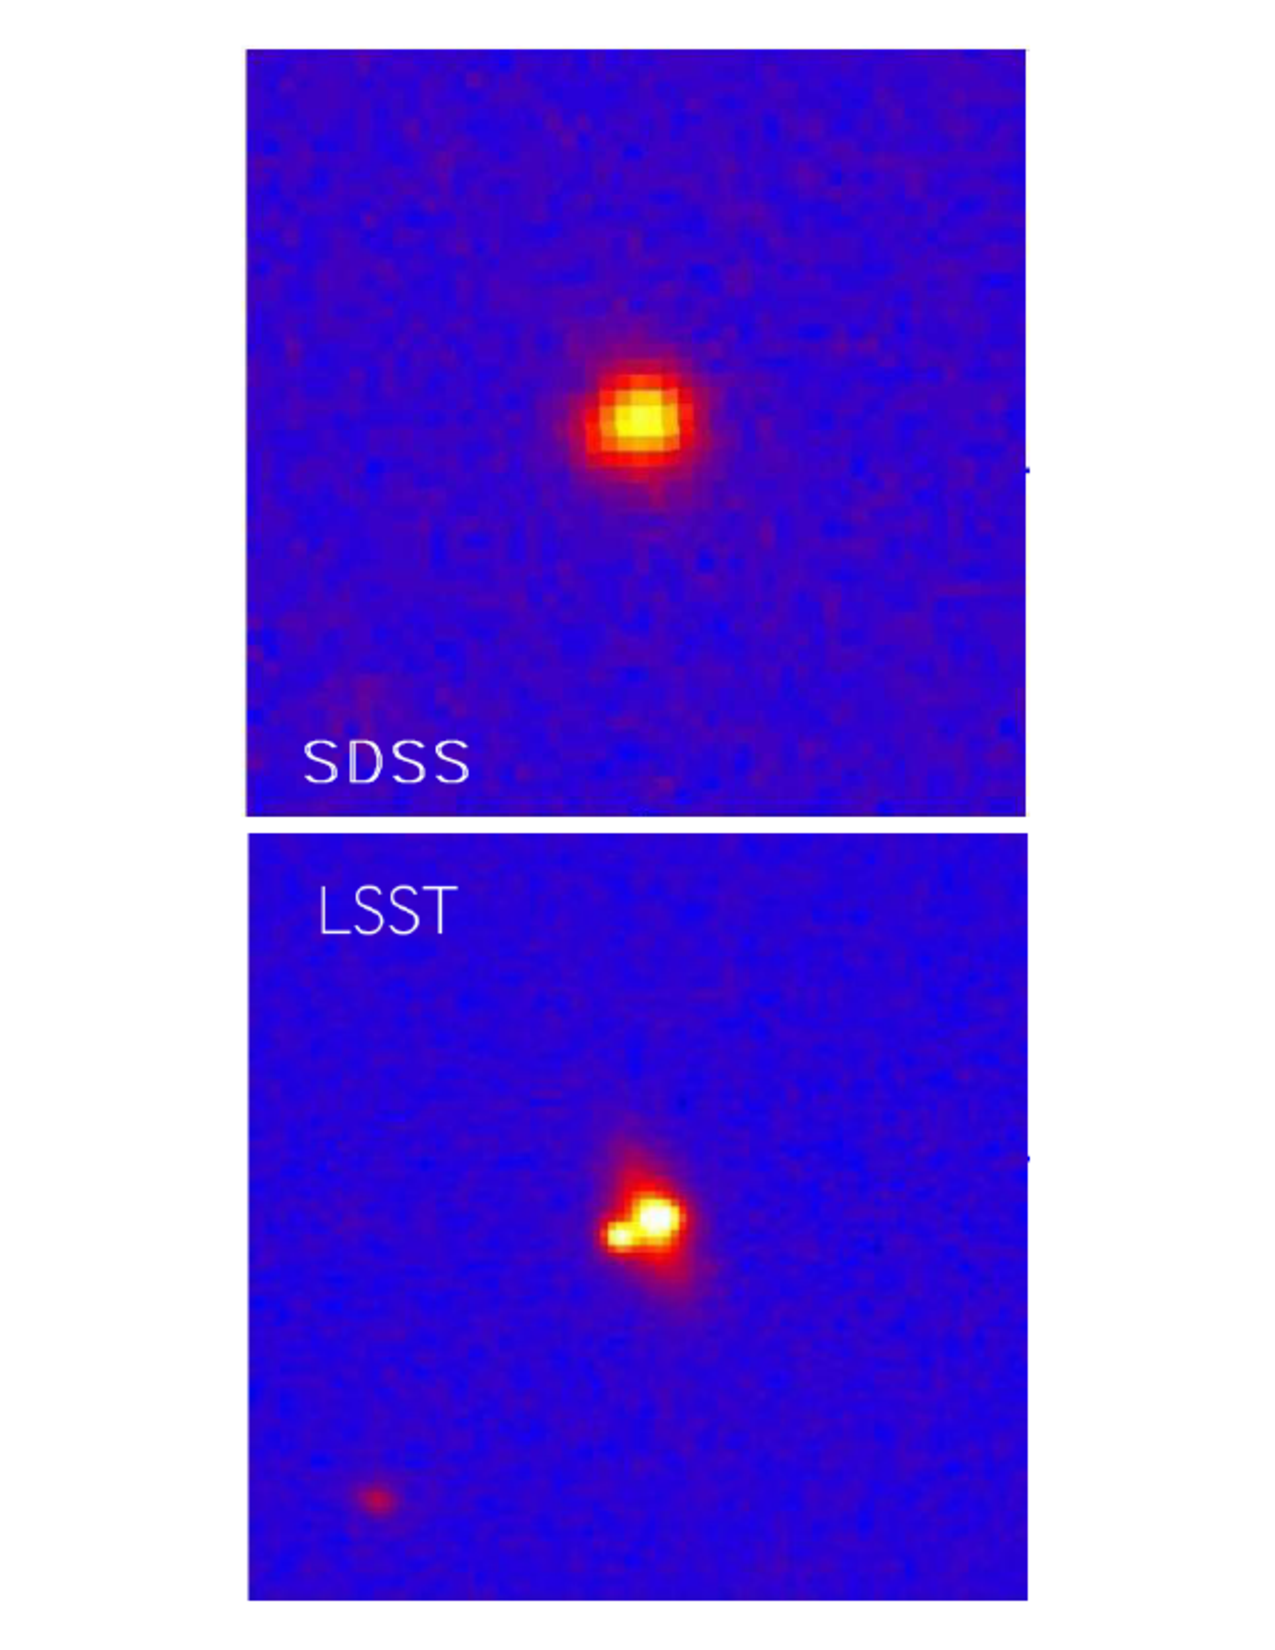
\includegraphics[width=0.47\textwidth,clip]{panels2}
\end{center}
\caption{A comparison of angular resolution for $20\times20$ arcsec$^2$ images obtained
by the SDSS (top, median seeing of 1.5 arcsec) and expected from LSST (bottom,
seeing of 0.7 arcsec). The images show a lensed SDSS quasar
\citep[SDSS J1332+0347,][]{2007AJ....133..214M}; the bottom image was taken with Suprime-cam at Subaru.
Adapted from \citet{2007AAS...21113707B}.}
\label{Fig:panels2}
\end{figure}
